\chapter{\label{chp:adaptinglegup}Adapting LegUp}
The main focuses of this project has been to resolve the issues encountered in \cite{holm2015pro}, to make LegUp able to generate Verilog more suited for ASIC implementation and synthesis. This chapter will describe the process of resolving these issues and other alterations that has been made in order to ease the creation of a framework for architectural exploration of hardware.
\section{Approach}
In the future works section of \cite{holm2015pro}, two different approaches to resolve the issues were proposed; post-processing and pre-processing. Both approaches have been explored, but the main section of solutions are based on the pre-processing alternative. The two following subsection will present the two approaches and give some reasoning to why one is chosen over the other.
\subsection{Post-processing}
With the post-processing approach, the idea is to alter the Verilog-code after it is generated, to make it more suitable for \gls{asic} implementations. This approach is easy to work with, as we can concentrate on a single file, the output Verilog file. The drawback of this approach is that you only have the information available in the Verilog file at hand, making it hard to add functionality to the tool.

There exist multiple parser tools for Verilog, for instance Verilog-Perl from VeriPool, a Verilog parser library for Perl \cite{verilogperl}, and pyverilog, a Hardware Design Processing Toolkit for Python \cite{Takamaeda2015Pyverilog}. These tools can be used to parse the Verilog file, to build module, signal, and port hierarchy, and easily add, alter, or remove objects.
\subsection{Pre-processing}
The pre-processing approach involves changing the libraries in LegUp that performs the HLS operations, like allocation, scheduling, RTL-generation and Verilog printing. This requires deep knowledge of the libraries and its connections, to find a good way to change the output. The large libraries is the main drawback of this approach. As LegUp is open-source, the possibilities of this approach are endless, but getting the necessary knowledge of the libraries takes time.
\subsection{The chosen approach}
As it looked like the easiest solution, the post-processing alternative were explored first. However, it were soon realised that the things that could be done easily with this approach, also could be done quite easily with the pre-processing approach. Some larger issues, for instance assigning values to outputs, were not easily solvable by using the post-processing method. The focus were therefore directed towards the pre-processing alternative. One advantage of this approach is that the original functionality of LegUp can be kept, while adding new functionality. The switching between original and altered versions are done using TCL-commands.

\section{TCL commands}
LegUp uses TCL commands for setting constraints and configure the HLS-flow. In order to not change the original implementation of LegUp, and to provide additional functionality, some new commands were added. New TCL-parameters can easily be added to LegUp by adding the parameter name to the array \textit{validParameters} and increasing the parameter \textit{NUM\_PARAMETERS} in the file \textit{LegupConfig.cpp}. The value of the parameter can then be read using the function call \verb!LEGUP\_CONFIG->getParameter("\%parameterName\%")! to get a string, or \verb!LEGUP\_CONFIG->getParameterInt("\%parameterName\%")! to get an integer. LegupConfig.h must be included to get access to LEGUP\_CONFIG. The most common use of TCL-parameters is to check whether a parameter is set, and perform some action based on this. Parameters can also be used to set values of variables. An example could be a parameter that decides if a designated top-module shall be generated or not. The parameter is define by adding the below line to the constraint file:

\begin{verbatim}
set_parameter PRINT_TOP_MODULE 1
\end{verbatim}
The parameter can then be used to decide if the Top-module should be printed:
\lstset{language=C++,style=Cstyle}
\begin{lstlisting}
if(LEGUP_CONFIG->getParameterInt("PRINT_TOP_MODULE") {
  printTop();
} else {
  printVerilogWithoutTop();
}
\end{lstlisting}

Another example is to use a parameter to set the name of the top-module. This can be used either for naming the top-module, or to select top-module in the simulation-settings. 
\begin{verbatim}
set_parameter TOP_MODULE_NAME "moduleName"
\end{verbatim}
\begin{lstlisting}
std::string topModuleName = "top"; // Default name
if(LEGUP_CONFIG->getParameter("TOP_MODULE_NAME") {
  topModuleName = LEGUP_CONFIG->getParameter("TOP_MODULE_NAME");
}
\end{lstlisting}
In the second example, the getParameter() function will return false if the parameter is not set.

Other TCL-commands can also be defined by adding the following line to the file \textit{LegupConfig.cpp}:
\begin{lstlisting}
Tcl_CreateCommand(interp,
                "set_custom_main_function",
                set_custom_main_function,
                legupConfig,
                0);
\end{lstlisting}
Here the second parameter is the TCL-command and the third parameter is the handler function that will be called when the TCL-command is encountered. In the handler function, arguments from the .tcl-file can be used to configure LegUp. As multiple arguments are supported, more advanced configurations can be performed with this alternative. The parameters that has been added to LegUp is described below.

\begin{description}
\item{\textbf{ASIC\_IMPLEMENTATION}} \hfill \\
This parameter is used to distinguish between the original version of LegUp and the altered version developed in this thesis. If this parameter is set, all extra features described in the following subsections will be applied to the generated design. If the parameter is not set, the unaltered edition of LegUp will be used to generate the output.
\item{\textbf{set\_custom\_main\_function}} \hfill \\
This parameter can be used to define inputs and outputs in the main module, as described in \cref{subsubsec:inoutparameter}. As this is not a simple TCL-parameters, it takes multiple arguments. The format of the input should be:
\begin{verbatim}
set_custom_main_function 
    input   7:0 inSignalA \
    input  31:0 inSignalB \
    output 31:0 outSignal \
    output  1:0 outSignalValid
\end{verbatim}
\item{\textbf{ENCLOSING\_WHILE\_LOOP}} \hfill \\
Main-function has enclosing while loop (for streaming inputs/outputs). Will generate \textit{iterationFinish}-signal each time an iteration of outer while loop is finished.
\item{\textbf{SEPARATE\_TB\_FILE}} \hfill \\
Parameter decides if testbench is printed in same file as design or in a separate file. The filename of the separate testbench-file will be \textit{test\_main.v}, according to Nordic Semiconductor's naming-convention, but this can easily be changed or made dynamic by setting the parameter \textit{SEPARATE\_TB\_FILENAME}.
\item{\textbf{SEPARATE\_TB\_FILENAME}} \hfill \\
Takes testbench filename as parameter and changes the default filename of the testbench output file to this name. Will not have any effect if \textit{SEPARATE\_TB\_FILE} is not set.
\item{\textbf{TB\_TESTCASE\_FILE}} \hfill \\
This parameter provides the filename of a file containing testcases for the testbench. The testcases will be automatically included into the testbench, as described in \cref{subsec:tbgen}. If the parameter is not set, no testcases will be added to the testbench.
\item{\textbf{REMOVE\_UNUSED\_LOCAL\_RAMS}} \hfill \\
By declaring input parameters as \textit{volatile}, a local RAM will be generated in the \textit{main}-module for each output signal we create. These RAMs is not used for anything useful and can therefore be removed to save area. If set, local RAMs in \textit{main} are removed \textbf{if} the value stored to the RAM is assigned to an output instead.
\end{description}

\section{\label{sec:removingmodules}Removing top-level and FPGA-specific modules}
As described in \cite{holm2015pro}, the output Verilog contains many module declarations not required or wanted in an ASIC implementation. This includes the module \textit{top}, \textit{memory\_controller}, \textit{circuit\_start\_control}, \textit{hex\_digits}, \textit{\%board\%} and \textit{main\_tb}. The modules \textit{memory\_controller} and \textit{main\_tb} are discussed in sections below, but it is desired to remove the other modules. Excess modules could easily be removed by parsing the generated Verilog-file, but the output can easily controlled with the use of TCL-parameters in the VerilogWriter-library of LegUp. When the parameter \textit{ASIC\_IMPLEMENTATION} is set, none of these modules are printed to the generated Verilog file.

\section{Removing memory controller}
One of the main issues with using LegUp for ASIC implementations, is that a global memory-controller for passing data between modules, are added to the design. With this architecture, values has to be added to the memory prior to the run or continuously during the run. This generate additional timing requirements and adds extra logic for handling these operations. Both to decrease the overhead, and to simplify the generated design, it is desirable to avoid this memory controller. A simple solution to this, is to set the parameter \textit{LOCAL\_RAMS} to 1. This parameter is already present in LegUp. Setting this parameter will prevent the global memory controller to be generated, as long as there are no variables used by multiple functions (global variables), or pointers that cannot be connected to a single functions after points-to analysis. Notice that no check on whether or not the memory controller is implemented in the design exist. Typically the memory controller will be instantiated in the \textit{top}-module, but as described in \cref{sec:removingmodules} this module is removed when the parameter \textit{ASIC\_IMPLEMENTATION} is set. This leads to no connections between the \textit{main}-module and the RAM-modules in the global memory controller, resulting in a failing circuit. It is therefore important to check that the global memory controller is not added to the design. Such a check could easily be implemented in the framework-script, described in \cref{sec:hlsscript}. By using the tool \textit{grep} to search for the line "\verb!module memory_controller!" in the generated Verilog-file, the user can be notified if the memory controller is found in the design.

\section{\label{subsec:inoutdecl}Declaring inputs and outputs}
Each function declared in the input C-code will be translated into a Verilog-module by LegUp. Since LegUp primarily is designed for implementing hardware accelerators for FPGAs, it does not handle inputs and outputs well to and from the \textit{top}-module. In an ASIC implementation, inputs and outputs are essential to most module design and must therefore be easy to implement. In a C-code written for execution on a computer, the input parameters to the \textit{main}-function is defined to be on the form "\verb!int main(int argc, char *argv[])!". This limits the possibility to declare inputs to the module with any data-type. To solve this problem, the flag \textit{-ffreestanding} has to be passed to the clang compiler frontend of LLVM. The compiler will then consider the C-code to contain a freestanding - not a hosted - environment. The types of inputs and return values defined in the \textit{main}-function has will thus be don't-care for the compiler. In LegUp, the flag can be passed to the compiler by adding it to the variable \textit{CLANG\_FLAG} in the file \textit{Makefile.config}. The solution that would have been used in a hosted environment is to use pointers for input and output parameters. This would however reintroduce the undesired memory controller.

Two different solutions for declaring inputs and outputs are considered and implemented. Both solutions are based on declaring both inputs and outputs as parameters to the \textit{main}-function.
\subsection{\label{subsec:inoutprefix}Name prefix}
The first solution is to use a prefix to distinguish between input- and output-parameters. To use a prefix that is seldom used in a variable name, the prefix is set to \textit{\_\_out\_}. Previously, LegUp assumed all function parameters were inputs, and added the signals to the RTLModule. This has been altered to check the name of the parameter and add it as an output reg if the name starts with \textit{\_\_out\_}, otherwise add it as an input. The pseudo-code of how inputs and outputs are handled are shown in \cref{alg:addInOut}. Here we assume that \textit{i} is a function parameter and \textit{rtl} is the RTLModule generated by the \textit{main}-function.

\begin{algorithm}
  \caption{\label{alg:addInOut}Pseudo-code of adding parameters to a module}
  \begin{algorithmic}[1]
    \Statex
    \State $sigName \gets i.getName()$
    \If{$sigName.startWith() = "\_\_out\_"$}
      \State $sigName \gets sigName.strip(\_\_out\_)$
      \State $i.setName(sigName)$
      \State $rtl.addOutReg(i)$
    \Else
      \State $rtl.addIn(i)$
    \EndIf
  \end{algorithmic}
\end{algorithm}

The advantage of this method is that it is simple to implement and easy to use, as the user only has to remember the name prefix when writing the functional specification. The name-prefix can also be useful in other sections of the program, as we will see later in section \ref{sec:assValueToOutput}. The disadvantage is that the name prefix needs to be used throughout the program. It would however be preferable to use a temporary variable in the program until the final value is calculated and ready to be assigned to the output. This will reduce the amount of times the name-prefix must be used. The name prefix will be stripped by LegUp, providing clean signal-names in the final Verilog-module.
\subsection{\label{subsubsec:inoutparameter}TCL-command}
The other alternative is to use a TCL-command to define the parameters as input or output. This enables the possibility to also define the size of the signal, but LegUp does not allow setting the size of a signals to a number of bits lower than the size of the defined type. This means that if a parameter is declared as an int in the C-program, LegUp does not allow for setting the RTLWidth of the signal to anything below 32 bit.

Inspiration for this method comes from the parameter \textit{set\_custom\_verilog\_function} already present in LegUp. This is used to add custom Verilog functions to the design. The TCL-command \textit{set\_custom\_main\_function} was added, which generate a vector with objects of the class CustomVerilogIO, each describing one input- or output-signal to the \textit{main}-module. By looping over the vector, each parameter can be added to the RTLModule based on this information. This part is quite similar to the above described name-prefix method. As this method does not provide any additional functionality, it is recommended to use the name-prefix method. The name-prefix method is also required together with another alteration described in \cref{subsec:llvmirparserprogram}.

\section{\label{sec:assValueToOutput}Assigning values to outputs}
In \cref{subsec:inoutdecl} two methods of declaring parameters as outputs in the generated module were presented. Unfortunately, assigning values to a input parameter is undefined behaviour in C. In the LLVM \gls{ir} output from the compiler, no assignment to any parameter is performed. The alternative of adapting the clang-compiler to threat name-prefixed input parameters as outputs were considered, but it would be time-consuming to dig into the clang-libraries as well. By disabling optimization of the \gls{ir} or declaring the output-parameter as \textit{volatile}, the assignment operation is present in the \gls{ir}-code. Unfortunately, the assignment in the \gls{ir}-code is not to a variable but to a local RAM module, generated for the parameter. No assignments to the output exists.

When disabling the optimization-passes in the compiler, some patterns were noticed that could provide useful information. The idea were to look for assignment information in the LLVM \gls{ir}-code, which could used in LegUp to assign the correct values to the output. To show how this information can be used to assign values to outputs, it is best to use a simple example. In \cref{lst:cllvmirparsercode}, a short C-code is listed. When running the pure-HW flow of LegUp, the human readable format of the LLVM \gls{ir}-code is output to a file called \textit{designName.ll}.
\lstset{language=C,style=Cstyle}
\begin{lstlisting}[caption={Simple C-code example for LLVM IR parsing},label=lst:cllvmirparsercode]
void main(int inDataA, int inDataB, volatile int __out_outData) {
  while (1) {
    __out_outData = inDataA * inDataB;
  }
  return;
}
\end{lstlisting}
\lstset{language=LLVM,style=LLVMStyle}
\begin{lstlisting}[caption={LLVM IR code for simple parsing example},label=lst:llvmirparsercode]
define void @main(i32 %inDataA, i32 %inDataB, i32 %__out_outData) #0 {
  %1 = alloca i32, align 4
  store volatile i32 %__out_outData, i32* %1, align 4
  br label %2

; <label>:2                                       ; preds = %2, %0
  %3 = mul nsw i32 %inDataA, %inDataB
  store volatile i32 %3, i32* %1, align 4
  br label %2
                                                  ; No predecessors!
  ret void
}
\end{lstlisting}
Lets analyze the LLVM \gls{ir} code output from compilation, shown in \cref{lst:llvmirparsercode}. On line 2 the temporary register \%1 is created. On line 3, the input parameter declared as volatile, \textit{\_\_out\_outData}, is stored to this register. On line 7, the calculated multiplication of the inputs \textit{inDataA} and \textit{inDataB} is stored to a new temporary register \%3. On line 8, the content of register \%3 is stored back to register \%1. This information can be exploited to create a program that traces stores, back to the original input parameter. In this example it is easy to see that the storing of the calculated multiplication easily can be traced back to the output \textit{\_\_out\_outData}, but in more complex programs, this tracing might not be that simple. One solution is to create a script that parses through the \gls{ir}-code and makes these connections. Notice that the parameter that should be an output \textbf{needs} to be declared as \textit{volatile}, if not the first allocation and store operations will be removed by link-time optimization passes. Optimization cannot be disabled, as this leads to temporary registers being used for all parameters rather than parameter-names, causing problems for streaming inputs described in \cref{sec:streamingio}.

When LegUp generates signals, they will be named by the convention:

\verb!functionName_labelNumber_registerNumber!. 

The example above will then create the signals \textit{main\_0\_1} from line 2 and \textit{main\_2\_3} from line 7. As the first line describes an \textit{alloc}-operation, \textit{main\_0\_1} will actually be implemented as a RAM-module. RAM-modules will be generated for all input-parameters declared as \textit{volatile}. This is good news, as this is needed for the program tracing assignments to outputs.
\subsection{\label{subsec:llvmirparserprogram}LLVM IR assignment parser program}
A program were created to parse the LLVM \gls{ir} generated by the compilation. The code for this program are written in the language C++. The reason for the language choice is merely that this was a familiar language for the writer of this thesis. The size of the program was not thought to be large enough for it to be beneficial to look into another language, given the limited amount of time available. In hindsight, a scripting language like Perl or Python could presumably be preferred for this kind of task. This section will explain in words and pseudo-code how the program works. The full source code of the parser program is included in \ref{lst:llvmirparserprogramcode} in the appendix. The program takes two command-line arguments when called, name of the input file and name of the output file. The input file should be the final LLVM \gls{ir} file generated by LegUp, named \textit{designName.ll}. The output filename can be anything, but the default filename used in LegUp for reading the output-file is \textit{LLVMParsed.log}. The program consist of two parts, the first part handles the reading and parsing of the input file, the second part is handling the generating of the output file. The program is created to only care about the main-function, as this is the module where it is vital to have multiple output signals. The program can easily be changed by altering the source code, if additional functionality is needed.

A pseudo-code describing the first part of the program is shown in \cref{alg:llvmparserpart1}. The parser starts by looking for the \textit{main}-function. When in the \textit{main}-function, the program looks for lines containing stores or labels. If a store is found, the source and target register of the store, together with the current label, is stored in separate vectors. If a new label is found, the label is set as the current label.

\algnewcommand\algorithmicto{\textbf{to}}
\algnewcommand\algorithmicand{\textbf{and}}
\begin{algorithm}
  \caption{Pseudo-code of input file handling in LLVM IR parser program
  \label{alg:llvmparserpart1}}
  \begin{algorithmic}[1]
    \Require{inFile and outFile should be passed as arguments}
    \Statex
    \If{$inFile.open()$}
    \State $currentLabel \leftarrow 0$
    \State $inMain \leftarrow false$
      \While{$inFile.getNextLine() \neq inFile.end()$}
        \If{$inMain$}
          \If{$lineStartWith() = "~~store"$}
            \State $newSource \leftarrow sourceRegisterFromLine$
            \State $newTarget \leftarrow targetRegisterFromLine$
            \State $sources.insert(newSource)$
            \State $targets.insert(newTarget)$
            \State $labels.insert(currentLabel)$
          \ElsIf{$lineStartWith() = ";~<label>:"$}
            \State $currentLabel \leftarrow labelNumberFromLine$
          \ElsIf{$lineStartWith() = "\}"$}
            \State $inMain \leftarrow false$
          \EndIf
        \ElsIf{$lineStartWith() = "define~\%type\%~@main"$}
          \State $inMain \leftarrow true$
        \EndIf
      \EndWhile
    \EndIf
  \end{algorithmic}
\end{algorithm}
A pesudo-code describing the second part of the program is shown in \cref{alg:llvmparserpart2}. A double for-loop is needed to check each target against each other target. The C-example above will store the values shown in \cref{tab:llvmirparservectors} in the vectors. 
\begin{table}[hbtp]
    \centering
    \begin{tabular}{ccc}
    \textbf{sources} & \textbf{targets} & \textbf{labels} \\
    \toprule
      \_\_out\_outData & 1 & 0 \\
      3 & 1 & 2 \\
    \bottomrule
    \end{tabular}
    \caption{Vector values after parser run}
    \label{tab:llvmirparservectors}
\end{table}
By comparing the first target against the second target in the table, it can easily be seen that the second source is stored to the same target as the first source. Notice that this program uses the name-prefix described in \cref{subsec:inoutprefix}. This method of declaring outputs is therefore required for the parser program to work. 
\begin{algorithm}
  \caption{Pseudo-code of output file handling in LLVM IR parser program
  \label{alg:llvmparserpart2}}
  \begin{algorithmic}[1]
    \If{$outFile.open()$}
    \State $done \leftarrow \{\}$
      \For{$i \leftarrow 0~\algorithmicto~targets.size()$}
        \For{$j \leftarrow 0~\algorithmicto~targets.size()$}
          \If{$targets[i] = targets[j]~\algorithmicand~i \neq j~\algorithmicand~sources[i] \notin done$}
            \State $newSource \leftarrow sourceRegisterFromLine$
            \State $newTarget \leftarrow targetRegisterFromLine$
            \State $done.insert(sources[j])$
            \If{$sources[i].lineStartWith() = "\_\_out\_"$}
              \State $parameterName \leftarrow sources[i].strip(\_\_out\_)$
              \State $outFile.print(parameterName)$
              \State $outFile.print(sources[j])$
              \State $outFile.print(labels[j])$
              \State $outFile.print(labels[i])$
              \State $outFile.print(targets[i])$
              \State $outFile.print("\backslash n")$ \Comment{$Newline$}
            \EndIf
          \EndIf
        \EndFor
      \EndFor
    \EndIf
  \end{algorithmic}
\end{algorithm}

The program will output the result of the tracing into the file with the name given as parameter to the program, with the given format:

\verb!"sources[i] sources[j] labels[j] labels[i] targets[i]"!

The output from the above example will then be:

\verb!"outData 3 2 0 1"!.

This implies that the signal \textit{main\_2\_3} should be assigned to the output \textit{outData}. The two last values, 0 and 1, are included as they will be used in a trick in \cref{subsec:assigningoutputsignals} to simplify the process of assigning signals to output ports.

Execution of the program is added to the Makefile, \textit{Makefile.common}, just before running the LegUp backend pass that generated Verilog output. The program is called by the line:
\begin{verbatim}
$(LEVEL)/LlvmParser.run $(NAME).ll LlvmParsed.log
\end{verbatim}

\subsection{\label{subsec:assigningoutputsignals}Assigning output signals}
As described in \cref{sec:legupclasses}, any RTLSignal that exist in an RTLModule can be found by calling the function \textit{find()}, with the name of the signal passed as a string parameter. A RTLSignal can have multiple drivers and conditions, and the i-th driver or condition can be found by calling \textit{getDriver(i)} and \textit{getCondition(i)}. The initial idea when the LLVM \gls{ir} parser program was created, was to find each of the signal and connect it to the correct output.

For every parameter to the function, the compiler will allocate a register and store the parameter value to this register. Whenever a store to a parameter is performed, this value will be stored to the first allocated register. In LegUp, the allocated register will be implemented as a RAM module and all stores to the parameter will be stored to this ram. This information can be exploited to easily assign values stored to this RAM to the output port instead.

Figure \ref{fig:assigningoutputs} tries to illustrate the problem with assigning outputs. In \cref{fig:assignoutputs1}, the module we would expect from the C-code in \cref{lst:cllvmirparsercode} is shown. The two inputs are multiplied together and output to \textit{outData}. In reality, what happens in the generated Verilog is shown in \cref{fig:assignoutputs2}. In \cref{fig:assignoutputs3}, the example is extended with an extra ADD module that stores to \textit{outData}. Instead of assigning the calculated values to the output, they are stored in a RAM module. In \cref{fig:assignoutputs3}, the current state is used to decide which signal is input to the RAM. The solution to this problem is shown in \cref{fig:assignoutputs4}. By "hijacking" the input signal to the RAM module and assigning it to the output, \textit{outData}, we get the expected functionality. 
\begin{figure}[hbpt]
        \centering
        \begin{subfigure}{0.49\textwidth}\centering%no!\hfill
                    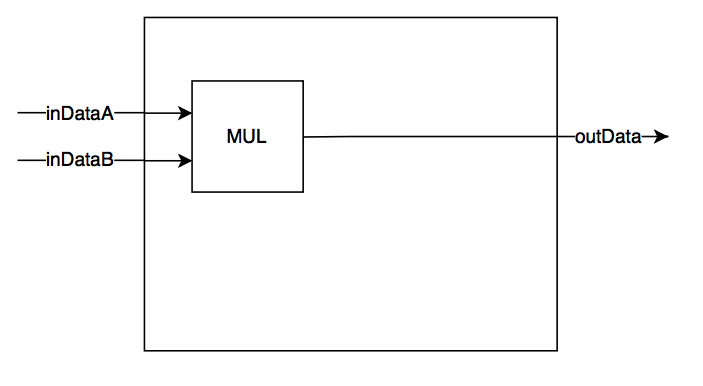
\includegraphics[width=\linewidth]{figs/OutputAssignment1.png}
                \caption{What we want to achieve}
  \label{fig:assignoutputs1}
       \end{subfigure}%
    \hfill
        \begin{subfigure}{0.49\textwidth}\centering
                    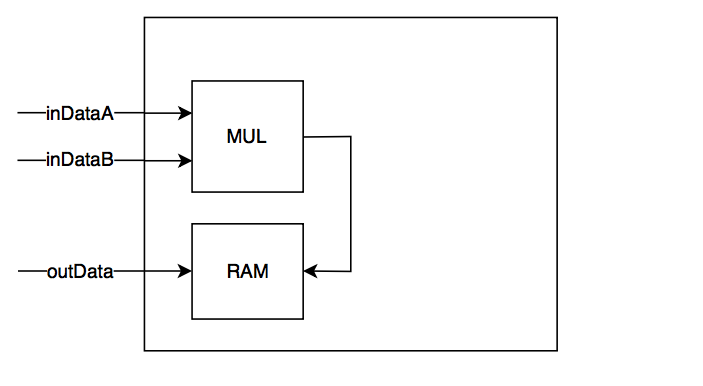
\includegraphics[width=\linewidth]{figs/OutputAssignment2.png}
                \caption{What the compiler/Legup thinks we want to achieve}
  \label{fig:assignoutputs2}
       \end{subfigure}%
    \hfill
        \begin{subfigure}{0.49\textwidth}\centering
                    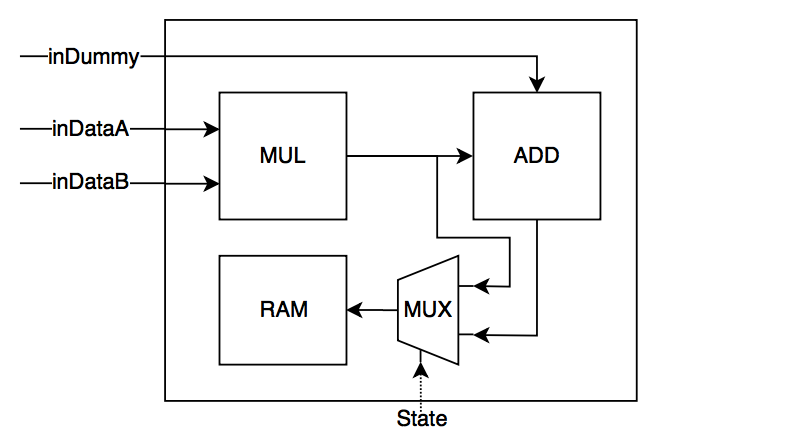
\includegraphics[width=\linewidth]{figs/OutputAssignment3.png}
                \caption{An example with multiple stores to \textit{outData}}
  \label{fig:assignoutputs3}
       \end{subfigure}%
    \hfill
        \begin{subfigure}{0.49\textwidth}\centering
                    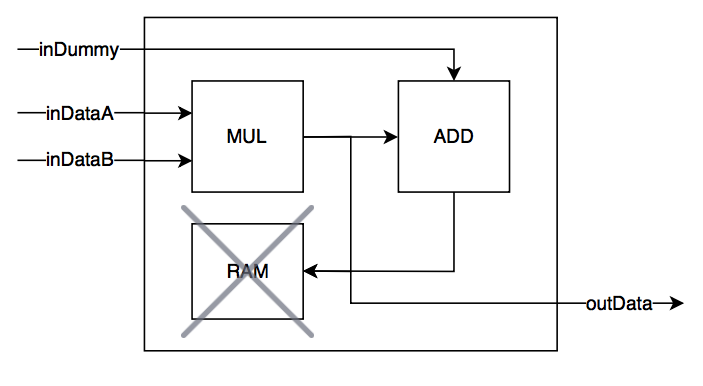
\includegraphics[width=\linewidth]{figs/OutputAssignment4.png}
                \caption{The solution}
  \label{fig:assignoutputs4}
       \end{subfigure}%
\caption{\label{fig:assigningoutputs}Problem with assigning values to output}
\end{figure}
The RAM module will be named by the same convention as signals, naming the RAM from the example \textit{main\_0\_1}. The data input-signal of the RAM module is named \textit{ramName\_in\_a}. This is the signal we want to "hijack". The "hijacking" is performed as described in \cref{alg:assignoutputsignals}. The name of the output ports are read from the file output from the LLVM \gls{ir} parser program, together with the name of the corresponding RAM modules. Each driver-condition pair in the input-signal of the RAM module, is added as a conditional driver to the output port.
\makeatletter
\let\OldStatex\Statex
\renewcommand{\Statex}[1][3]{%
  \setlength\@tempdima{\algorithmicindent}%
  \OldStatex\hskip\dimexpr#1\@tempdima\relax}
\makeatother
\begin{algorithm}
  \caption{Pseudo-code of assigning values to outputs
  \label{alg:assignoutputsignals}}
  \begin{algorithmic}[1]
    \For{$i \leftarrow 0~\algorithmicto~outputPorts.size()$}
      \State $outputPort \gets find(output~signal~name)$
      \State $ramSignal \gets find(RAM~module~inData~signal)$
      \For{$j \gets 0~\algorithmicto~ramSignal.getNumDrivers()$}
        \State $outputPort.addCondition(ramSignal.getDriver(j),$
        \Statex[9] $~~~~ramSignal.getCondition(j))$
      \EndFor
    \EndFor
  \end{algorithmic}
\end{algorithm}

\subsection{Removing local RAMs}
As described in \cref{sec:assValueToOutput}, each parameter declared as \textit{volatile} will generate a RAM module. After reassigning the stores to the output port, the generated RAM modules are no longer needed. These RAM modules can be removed to save area and reduce power consumption. To make this operation optional, the TCL-parameter \textit{REMOVE\_UNUSED\_LOCAL\_RAMS} were added. By setting this parameter, the local RAM modules will be removed. All local RAMs are stored together with its corresponding function (from the C-code) in a variable, \textit{isLocalFunctionRam}. To remove the RAM, it is simply removed from this variable. In addition to removing the RAM module, all signals to and from the RAM needs to be removed as well. Notice that only the RAMs generated by output parameters are removed from the \textit{main}-module. RAM modules can also be generated by arrays and other large data structures, but these will not be removed. This method of removing the RAMs does not remove the states for allocation and stores to the RAMs present in the FSM generated by LegUp. 

\section{\label{sec:streamingio}Streaming inputs/outputs}
For most module designs to be useful and fast, it must be able to continuously take new inputs and generate outputs, without having to start and stop the entire module each time, with all the overhead in time this would require. The way LegUp is designed, functions are used as hardware accelerators, meaning it gets some input, performs some calculations and then outputs the result. The module is then finished and will not run again until next time the accelerated function is called. For this approach to work for an ASIC implementation, a top module would need to be created to assign new inputs and start the module again once it is finished with the last iteration. If the output-value is used in the next run, a feedback loop needs to be added to pass the result back to the new inputs. The concept is shown in \cref{fig:steamininputstop}. This solution would be hard to implement and would create extra overhead, both in terms of speed and area of the design. Another solution would be to add a while loop inside the \textit{main}-function of the C-code to make the program run continuously. The initial problem with this approach is that to return a value from the function, the \textit{return}-statement is used. Calling \textit{return} will cause the program to terminate, which is not desirable. With the method implemented in \cref{sec:assValueToOutput}, it is no longer necessary to call \textit{return} to output a value. This while-loop method can therefore be used with this altered version of LegUp.

\begin{figure}[hbpt]
\centering
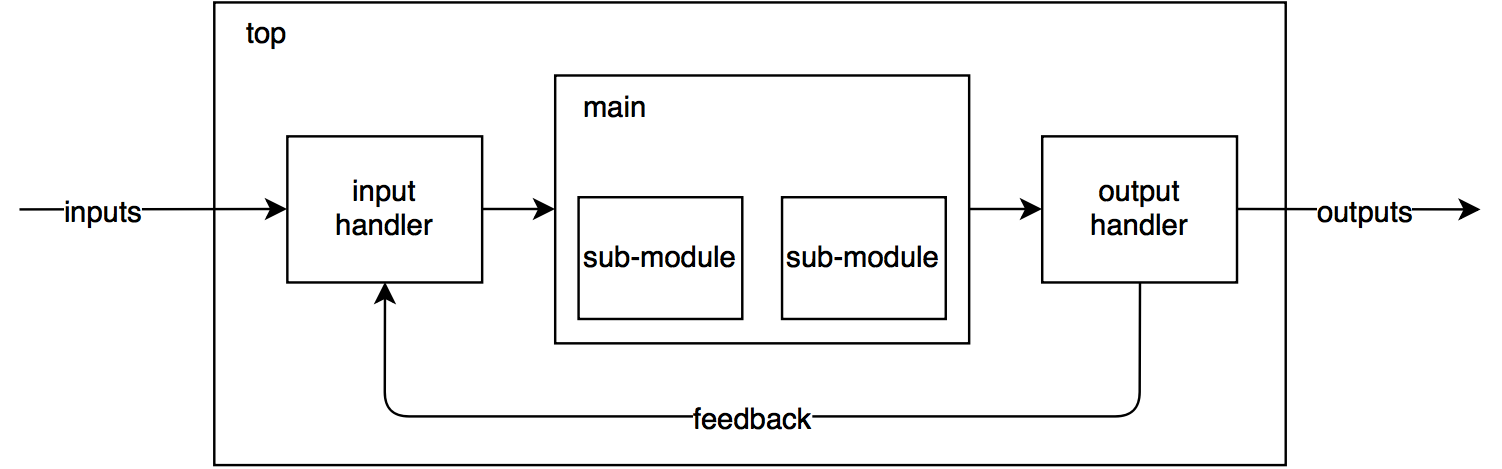
\includegraphics[width=\textwidth]{../figs/StreamingInputs.png}
\caption{\label{fig:steamininputstop}Top-level concept for streaming inputs and outputs}
\end{figure}

With this solution, some new issues arise. First we need a way to stop the module if all calculations are finished. This can easily be handled by adding a input parameter to the main function in the C-program, lets call it \textit{done}, which is used as condition for running the while-loop. This parameter will then correspond to a signal in the Verilog-module that can be used to terminate the module. No alterations to LegUp is performed to resolve this issue, as it can be resolved manually by the user. This signal could potentially be integrated to the Verilog generation in LegUp, but this would require major alterations to the libraries and the generated data-flow.

Secondly, we need a way to know when an output has valid data. A simple solution here is to generate a valid-flag for each output signal. These flags are created simultaneously with the outputs being connected to the driving signals, as described in \ref{sec:assValueToOutput}. The signals shall be valid only in the first clock cycle after the output signal has changed. To achieve this, two condition signals has to be created, one when the output is valid, and one when the output is not valid. The valid condition shall be set in any state where the output signal is assigned. This means that the conditions used to set the RAM module's data input-signal can be used. The not-valid signal should be set in all other states. To generated the valid-signal is straightforward, as the condition-signals for storing values to the RAM is already generated by LegUp. These conditions can be copied from the RAM-signal and added to the output-valid signal as conditional drivers. The not-valid signal is a bit more tricky to generate. By creating an RTLOp-signal that ANDs together all the valid states, and creating a second RTLOp-signal that NOTs this signal, the desired not-valid signal is created. Figure \ref{fig:validsignals} illustrates how the signal is generated. The tricky part arises from the AND-operation only being able to take two operands, making it hard to create code handling special cases of few and odd number of valid states. The source code of how this is handled is included in \cref{sec:validsinglssourcecode}.

\begin{figure}[hbpt]
\centering
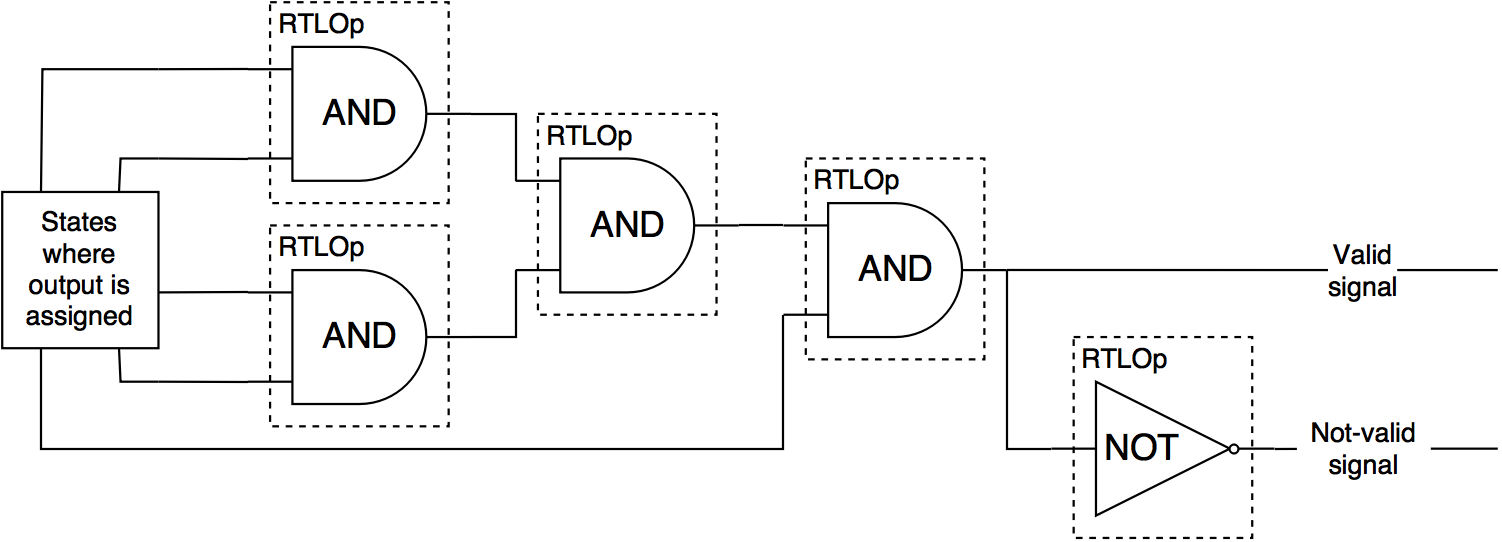
\includegraphics[width=\textwidth]{../figs/ValidSignals.png}
\caption{\label{fig:validsignals}Generating not-valid signal.}
\end{figure}

As each output can be valid at different times, and also multiple times during a loop, a third issue needs to be handled. A way to know when an iteration of the loop is finished must be added. A flag, \textit{iterationFinish}, can be added by setting the parameter \textit{ENCLOSING\_LOOP} in the constraint file. The flag will be set each time the loop condition-check is performed (except the first time). If the code is divided into three parts, pre-loop, loop, and post-loop, the implementation of this solution can be simplified a bit. By not allowing any operations, except return, to be executed in the post-loop part, as shown in \cref{lst:enclosingloopc}, the flag needs only be set in the state preceding the final state of the FSM.
\lstset{language=C,style=Cstyle}
\begin{lstlisting}[caption={Sectioning of a program with enclosing while-loop},label=lst:enclosingloopc]
void main( int done ) {
  //Pre-loop: Variable setup etc. can be done here.
  while(done == 0) {
    //Loop: Functional operations are performed here
  }
  //Post-loop: No operations can be done here.
  return;
}
\end{lstlisting}
The \textit{iterationFinish}-flag is set to zero in all other states. This is done by adding an RTLOp-signal that NOTs the condition for setting the flag high. This RTLOp-signal is added as a conditional for driving the flag low. The source code of this is listed in \cref{sec:iterationfinishsourcecode}.

\section{Signal sizes}
A problem with writing the functional specification in C is that C have no built-in support for bit-sizes. Data types of sizes 1, 8, 16, 32 and 64 bits are defined, but if you want to declare a signal of any other bit-width, like you often do in hardware design, this is not possible. The problem with over-sized signal sizes is that larger circuits will be generated in order to handle the calculation of the expected extra bits. Two solutions were looked upon for solving this issue; bit-packed structs and bit-width attributes. In C it is supported to define a variable in a struct to be any given number of bits. The thought behind this feature is to allow storing multiple small variables in the memory space occupied by the entire struct. In the example shown in \cref{lst:structpacking} the struct \textit{s} will occupy 12 bytes, as one int equals 4 bytes, while the struct \textit{t} will occupy 3 bytes, as the total defined bit-width is 23 bits.
\begin{lstlisting}[caption={Struct bit-packing example},label=lst:structpacking]
struct s {
  int a;
  int b;
  int c;
}__attribute__((packed));

struct t {
  int a:1;
  int b:15;
  int c:7;
}__attribute__((packed));
\end{lstlisting}
There are two issues with this solution; assigning values to a variable in a struct takes much more typing than other variables, even if the struct only contains a single variable, and structs are not supported by the inferred RAMs generated by LegUp. This means that if structs are used in the design, \textit{altsyncram}-modules are generated in place of inferred RAMs.

The other alternative that has been explored is to use a attribute that sets the bit-width of a variable. By adding \verb!__attribute__((bitwidth(N)))! to the end of the variable declaration, where \verb!N! is the number of bits in the signal, the compiler can define the signal size based on this attribute. Implementation of this attribute were suggested as an addition to \textit{llvm-gcc}, the GCC frontend compiler for LLVM, in 2007 \cite{bitwidthattr}, but unfortunately it were discarded in 2010. This attribute would allow for defining new data types for each size, and using them as standard data types:
\begin{lstlisting}
typedef int __attribute__((bitwidth(2))) int2;
typedef int __attribute__((bitwidth(4))) int4;
typedef int __attribute__((bitwidth(25))) int25;

int2 a = 3;
int4 b = 8;
int25 c = 2502;
\end{lstlisting}
which could be translated into the following in the LLVM \gls{ir}:
\begin{lstlisting}
@a = global i2 3, align 4
@b = global i4 8, align 4
@c = global i25 2502, align 4
\end{lstlisting}
The align value could be lower, depending on the number of bits/bytes allocated to each temporary register. This solution is possible to implement in theory, but it would require changing both the clang compiler frontend for LLVM and the LegUp backend pass. Due to the estimated amount of time this alterations would require, this issue have not been resolved. For this thesis it is not vital that we can set exact signal sizes, as long as we use the same sizes in both C and Verilog code to get a fair comparison.

\section{\label{subsec:tbgen}Testbench generation}
The original version of LegUp generates a basic testbench shell, but this is very static. It is also and incorporated into the same file as the \gls{rtl}-design, making it impractical to use in the desired framework. The generated testbench consists of a testbench module, \textit{main\_tb}, which instantiate the \textit{top}-module, \textit{top}, and sets \textit{reset}, \textit{start} and \textit{waitrequest} flags. The input and output signals in the top module does not contain custom signals from the \textit{main}-module, and in an ASIC implementation we are not interested in the memory controller and additional modules declared/instantiated in the top module. The solution then, became to instantiate the \textit{main}-module instead and add each input or output by iterating over the ports in the \textit{main}-module. By setting the TCL-parameter \textit{SEPARATE\_TB\_FILE}, the testbench will be output to a separate file from the \gls{rtl}-design. The source code of how the testbench-generation is performed is listed in \cref{sec:tbgenerationsourcecode}.

As the testbench does not come with any form of testcases or applied signals, the testbench generator is extended to input Verilog code from a file specified by the TCL-parameter \textit{TB\_TESTCASE\_FILE}. This allows the user to specify testcases in this file, that will be automatically inserted into the testbench file. The code will be placed inside the testbench-module, but not inside any procedural blocks. This allows the user to add the preferred procedural block in the specified testcase file. An example testcase file can then be:

\lstset{language=Verilog, style=Verilogstyle}
\begin{lstlisting}
always @(iterationFinish) begin
  if (iterationFinish == 1) begin
    $display("At t=%t, Loop iteration finished", $time);
  end
end
\end{lstlisting}
or
\begin{lstlisting}
initial begin
    inData <= 100;
    @(posedge clk)
    inData <= 0;
    @(posedge clk);
    $display("At t=%t, outData=%d", $time, outData);
end
\end{lstlisting}
This insertion of testcases, enables the script to automatically run HLS and thereafter run simulation using the generated design and testbench.

\section{Coding constraints}
Due to the described alterations to the LegUp libraries, some guidelines need to be followed when writing the functional specification, to ensure correct output. The following subsections will describe these guidelines.
\subsection{Structs}
To support structs, byte-enable must be supported by the RAM or ROM module used to store the data. The RAM and ROM modules inferred by LegUp does not support byte-enable, resulting in struct support not being present when writing the functional specification. If structs are used in the code, LegUp will use an altsyncram-module instead of inferring RAMs. The altsyncram-module is not supported by the IC-compiler tool-flow used at Nordic Semiconductor for synthesis, and inferred RAM-modules must therefore be used. 
\subsection{Pointers}
Pointers are used to reference an object in memory, opposed to passing a copy of the actual object between function. This reduces both CPU-time and memory-space, as objects does not need to be copied every time it is used, and makes it possible to alter a memory object directly without implicit load and store operations. As the memory controller used to pass data between different modules are unwanted in an ASIC implementation, support for pointers are limited to use inside the function where the pointer is declared. This limitation is a big drawback with this altered version of LegUp.
\subsection{Arrays}
Arrays can be used in the programs to some extent, but if the arrays get too large or too many arrays are instantiated, LegUp will implement them as RAMs inside the global memory controller. The reason for this is that arrays in C basically is a pointer to the array type. When the point-to analysis cannot determine that a single function use the array, it is automatically implemented as a global RAM.
\subsection{Inputs and outputs}
The implemented method of adding inputs and outputs to the module is not ideal. The need for using name-prefixes when writing the C-code puts more of the work on the coder, and draws the input further away from the standard ANSI-C that were intended as the input language. If using a while loop for supporting streaming inputs and outputs, it is not possible to do calculations after the loop, as this will break generation of the \textit{iterationFinish}-flag. Not being able to specify signal sizes also limits what designs can be created using the tool. All these limitations has to be taken into consideration when writing the functional specification, to make sure the design is supported by the tool-flow and framework.